\documentclass[11pt]{article}
\usepackage[utf8]{inputenc}
\usepackage{amsmath, amssymb}
\usepackage{geometry}
\usepackage{listings}
\usepackage{xcolor}
\usepackage{graphicx}
\usepackage{tabularx}
\usepackage{booktabs}
\usepackage{hyperref}

\geometry{a4paper, margin=1in}

\definecolor{codegray}{rgb}{0.5,0.5,0.5}
\definecolor{codepurple}{rgb}{0.58,0,0.82}
\definecolor{backcolour}{rgb}{0.95,0.95,0.92}

\lstset{
    language=Python,
    backgroundcolor=\color{backcolour},
    commentstyle=\color{codegray},
    keywordstyle=\color{magenta},
    stringstyle=\color{codepurple},
    basicstyle=\ttfamily\small,
    breaklines=true,
    showstringspaces=false
}

\title{Physics Lab: Ray Tracing and Geometrical Optics \\ \large Problem Set \& Implementation Guide}
\author{VB}
\date{\today}

\begin{document}

\maketitle

\section*{Problem 0: Start the engine}

Consider the files given.
\begin{center}
\renewcommand{\arraystretch}{1.5}
\begin{tabularx}{\textwidth}{@{} >{\bfseries\raggedright\arraybackslash}p{5.5cm} X @{}}
\toprule
\textcolor{blue}{Filename} & \textcolor{blue}{Purpose} \\ \midrule
\multicolumn{2}{@{}l}{\textbf{Direct Interaction}} \\ \midrule
\lstinline|implementation_tasks.py| & \textcolor{red}{Here you write your code.} Contains the core physics and geometry logic (intersections, refraction, and normals) intended for student implementation. \\
\lstinline|lab_dashboard.py| & \textcolor{red}{This file you run.} A dedicated educational sandbox for debugging individual physics levels through an interactive UI. This is your main interaction point\,-- other scripts can be started from here.\\
\lstinline|optic_bench.py| & \textbf{May be run standalone after you solve levels 1-7.} The main simulation engine; allows for the creation and management of simple optical systems, and uses the math you implement in \lstinline|implementation_tasks.py|. \\
\lstinline|levels/level_*.py| & Unittests and graphical representation for each specific problem. \textbf{Can be run standalone.} You can use \lstinline|python levels/level_*.py| for the graphical debugger or \lstinline|python levels/level_*.py --no-graphics| for unittests only. \\ \midrule
\multicolumn{2}{@{}l}{\textbf{Under the Hood}} \\ \midrule
\lstinline|levels/base_level.py| & Base class for graphical debuggers.\\
\mbox{\lstinline|ray_tracer.py|}, \mbox{\lstinline|lens_object.py|}, \mbox{\lstinline|ray.py|}, \mbox{\lstinline|ray_source.py|}, \mbox{\lstinline|lens_architect.py|}, \mbox{\lstinline|inspector.py|}, \mbox{\lstinline|io_manager.py|} & Needed for Optic Workbench. These manage the global state, perform recursive ray tracing, save/load optical system, and provide UI for the final simulation. \\
\bottomrule
\end{tabularx}
\end{center}


Run the file \lstinline|lab_dashboard.py|. You should see the window as follows
\begin{center}
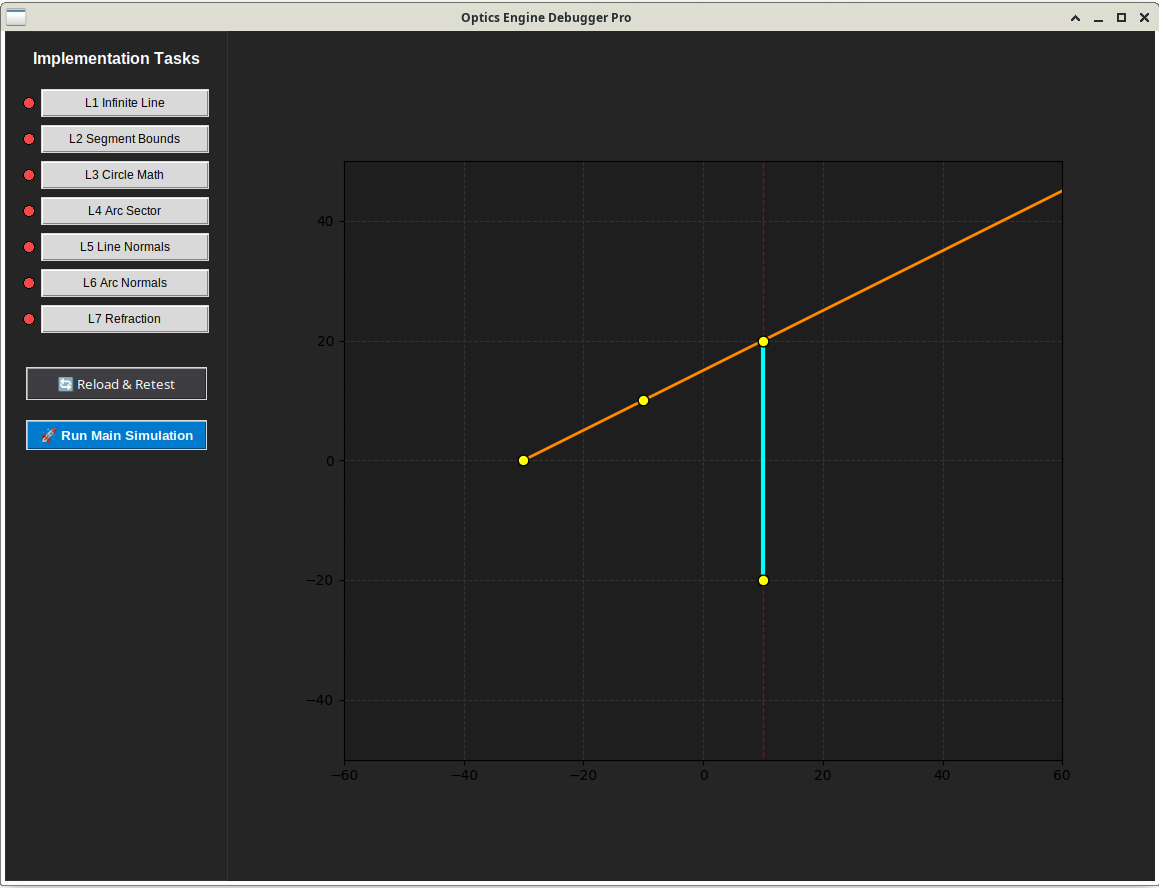
\includegraphics[width=0.8\textwidth]{lab_dashboard_1}
\end{center}


Now use any editor to open the file \lstinline|implementation_tasks.py|. You should see API for functions you should implement.
\begin{lstlisting}
import numpy as np

# =============================================================
#  STUDENT IMPLEMENTATION (ASSIGNMENTS 1-4)
# =============================================================

CONST_EPSILON = 1e-5

def intersect_line_infinite(ray_origin, ray_dir, p1, p2):
    pass

def intersect_segment(ray_origin, ray_dir, p1, p2):
    pass

<<<< MORE CODE >>>>
\end{lstlisting}


Now proceed with the following problems. First solve the math part so you get the equation. Than implement. After implementation press "Reload \& Retest" button and see if the bulb near the appropriate task becomes green, if not there are probably some issues with your implementation. Click the button with the appropriate task to get some visuals, drag elements on the scene and see where your point is, this should help debugging.

\section*{Problem 1: Linear Intersection (Infinite Line)}

\subsubsection*{Mathematical part}
\textbf{Given:} A light ray starting at origin $\mathbf{O}$ with a unit direction vector $\vec{d}$, and an infinite line passing through two given points $\mathbf{P}_1$ and $\mathbf{P}_2$. \\
\begin{center}
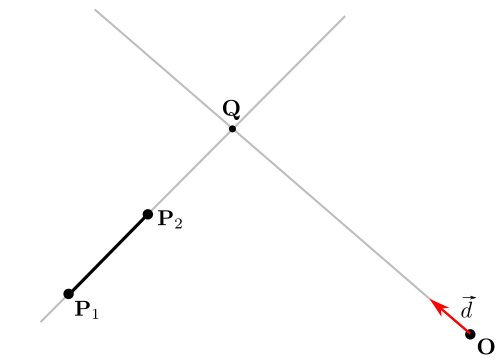
\includegraphics[width=0.5\textwidth]{lines_intersection}
\end{center}
\textbf{Derive:} The intersection point of the ray and this line $\mathbf{Q}$. \textbf{Hint:} use vector representation $\vec{l}(t) = t \vec{u} + \vec{v}$ to write equations for lines.\\

\subsubsection*{Implementation part}
\textbf{Implement:} a function \lstinline|intersect_line_infinite(ray_origin, ray_dir, p1, p2)| that returns intersection point $\mathbf{Q}$ as a \lstinline|numpy.array| with two coordinates. If the ray does not intersect the line, return \lstinline|None|.
\begin{center}
\renewcommand{\arraystretch}{2.0}
\begin{tabular}{r | c | c | c | c | c}
\toprule
\textbf{Math Symbol} & $\mathbf{O}$ & $\vec{d}$ & $\mathbf{P}_1$ & $\mathbf{P}_2$ & $\mathbf{Q}$ \\ \midrule
\textbf{Argument} & \lstinline|ray_origin| & \lstinline|ray_dir| & \lstinline|p1| & \lstinline|p2| & \lstinline|return| \\ \midrule
\textbf{Type} & \lstinline|np.array| & \lstinline|np.array| & \lstinline|np.array| & \lstinline|np.array| & \lstinline|np.array| or \lstinline|None| \\
\bottomrule
\end{tabular}
\end{center}
\textbf{Test:} Press "Reload \& Retest" button and see if the bulb near the appropriate task becomes green, if not there are probably some issues with your implementation. Press "L1 Infinite Line" button in the visual debugger window. Move different points and see how the intersection point is displayed. Fix any bugs if you see inconsistencies, point disappears when it shouldn't or appears in the wrong place.

\section*{Problem 2: Boundary Logic (The Segment)}

\subsubsection*{Mathematical part}
\textbf{Given:} A light ray starting at origin $\mathbf{O}$ with a unit direction vector $\vec{d}$, and a segment defined by its endpoints $\mathbf{P}_1$ and $\mathbf{P}_2$. \\
\textbf{Derive:} Conditions that the intersection point $\mathbf{Q}$ of the ray and the line passing through $\mathbf{P}_1$ and $\mathbf{P}_2$ lies on the segment $\overline{P_1P_2}$. \textbf{Hint:} you can use your previous result, just think regarding restrictions.\\

\subsubsection*{Implementation part}
\textbf{Implement:} a function \lstinline|intersect_segment(ray_origin, ray_dir, p1, p2)| that returns intersection point $\mathbf{Q}$ as a \lstinline|numpy.array| with two coordinates. If the ray does not intersect the segment, return \lstinline|None|. \textbf{Hint:} call your function for the line to get the point. Test that the point is on the segment.

\begin{center}
\renewcommand{\arraystretch}{2.0}
\begin{tabular}{r | c | c | c | c | c}
\toprule
\textbf{Math Symbol} & $\mathbf{O}$ & $\vec{d}$ & $\mathbf{P}_1$ & $\mathbf{P}_2$ & $\mathbf{Q}$ \\ \midrule
\textbf{Argument} & \lstinline|ray_origin| & \lstinline|ray_dir| & \lstinline|p1| & \lstinline|p2| & \lstinline|return| \\ \midrule
\textbf{Type} & \lstinline|np.array| & \lstinline|np.array| & \lstinline|np.array| & \lstinline|np.array| & \lstinline|np.array| or \lstinline|None| \\
\bottomrule
\end{tabular}
\end{center}
\textbf{Test:} Press "Reload \& Retest", than "L2 Segment Bounds" buttons in the visual debugger window. Ensure unittests are passing. Move different points in visual debugger and ensure your code works appropriately.


\section*{Problem 3: Quadratic Geometry (Circle)}

\subsubsection*{Mathematical part}
\textbf{Given:} A light ray starting at origin $\mathbf{O}$ with a unit direction vector $\vec{d}$, and a circle defined by its center $\mathbf{C}$ and radius $R$. \\
\textbf{Derive:} The intersection points $\mathbf{Q}_1$ and $\mathbf{Q}_2$ of the ray and the circle. Define them in way $\mathbf{Q}_1$ is \textbf{always closer} to the ray source than $\mathbf{Q}_2$. \textbf{Hint:} substitute the ray equation $\mathbf{r}(t) = \mathbf{O} + t\vec{d}$ into the circle equation $\|\mathbf{r} - \mathbf{C}\|^2 = R^2$ and solve the resulting quadratic equation for $t$. Note that the discriminant is always a positive number.

\subsubsection*{Implementation part}\textbf{Implement:} a function \lstinline|intersect_circle(ray_origin, ray_dir, center, radius)| that returns a list of intersection points $\mathbf{Q}_1$ and $\mathbf{Q}_2$ as \lstinline|numpy.array| objects. Make sure that \textbf{the point closer to the ray source precedes in the list}. If no intersection exists, return an empty list \lstinline|[]|. If there is only one intersection point, you can either return a list containing only that point, or a list containing its two copies\,--- both cases will be valid.
\begin{center}
\renewcommand{\arraystretch}{2.0}
\begin{tabular}{r | c | c | c | c | c}
\toprule
\textbf{Math Symbol} & $\mathbf{O}$ & $\vec{d}$ & $\mathbf{C}$ & $R$ & $\{\mathbf{Q}_1, \mathbf{Q}_2\}$ \\
\midrule\textbf{Argument} & \lstinline|ray_origin| & \lstinline|ray_dir| & \lstinline|center| & \lstinline|radius| & \lstinline|return| \\
\midrule
\textbf{Type} & \lstinline|np.array| & \lstinline|np.array| & \lstinline|np.array| & \lstinline|float| & \parbox{5cm}{\lstinline|[np.array, np.array]| or\\ \lstinline|[np.array]| or \lstinline|[]|} \\
\bottomrule
\end{tabular}
\end{center}
\textbf{Test:} Press "Reload \& Retest", than "L3 Circle Math" buttons in the visual debugger window. Ensure unittests are passing. Move different points in visual debugger and ensure your code works appropriately. \textbf{Note: only the first point from the list is displayed in the debugger.} This is to help you understand whether you return points in the correct order.


\section*{Problem 4: Angular Sector (The Arc)}

\subsubsection*{Mathematical part}
\textbf{Given:} A light ray starting at origin $\mathbf{O}$ with a unit direction vector $\vec{d}$, and an arc defined by center $\mathbf{C}$, radius $R$, central axis unit vector $\vec{a}$, and the cosine of the \textbf{half}-aperture angle $\cos(\phi)$. \\
\textbf{Derive:} The condition that an intersection point $\mathbf{Q}$ lies within the angular sector of the arc (see image below). \textbf{Hint:} use the dot product between the normalized vector $(\mathbf{Q} - \mathbf{C})$ and the axis $\vec{a}$.

\begin{center}
 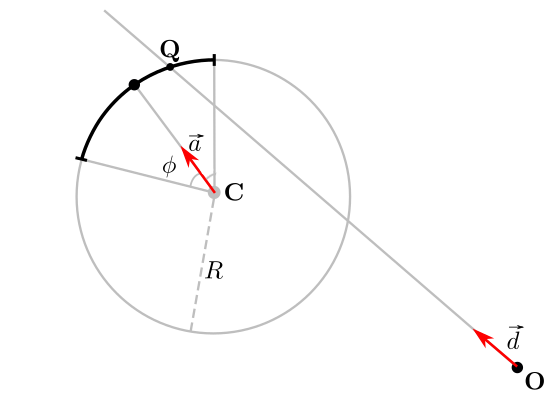
\includegraphics[width=0.5\textwidth]{arcs}
\end{center}


\subsubsection*{Implementation part}
\textbf{Implement:} a function
\begin{center}
\lstinline|intersect_arc(ray_origin, ray_dir, center, radius, axis, cos_half_angle)|
\end{center}
 that returns \textbf{the nearest} valid intersection point $\mathbf{Q}$ as a \lstinline|numpy.array|. Use the fact that \lstinline|intersect_circle| function returns points in order from closer to the ray source to further. If no point on the arc is hit, return \lstinline|None|. \textbf{Hint:} call your circle function and filter the results by the angular condition. If two points are left, check which one is hit first.
\begin{center}
\renewcommand{\arraystretch}{2.0}
\begin{tabular}{| c | c | c | c | c | c | c |}
\toprule
$\mathbf{O}$ & $\vec{d}$ & $\mathbf{C}$ & $R$ & $\vec{a}$ & $\cos(\phi)$ & $\mathbf{Q}$ \\
\midrule
\lstinline|ray_origin| & \lstinline|ray_dir| & \lstinline|center| & \lstinline|radius| & \lstinline|axis| & \lstinline|cos_half_angle| & \lstinline|return| \\
\midrule
\lstinline|np.array| & \lstinline|np.array| & \lstinline|np.array| & \lstinline|float| & \lstinline|np.array| & \lstinline|float| & \lstinline|np.array| or \lstinline|None| \\
\bottomrule
\end{tabular}
\end{center}
\textbf{Test:} Press "Reload \& Retest", than "L4 Arc Sector" buttons in the visual debugger window. Ensure unittests are passing. Move different points in visual debugger and ensure your code works appropriately.


\section*{Problem 5: Surface Orientation (Segment Normal)}

\subsubsection*{Mathematical part}
\textbf{Given:} An incident unit direction vector $\vec{d}$, and a segment defined by its endpoints $\mathbf{P}_1$ and $\mathbf{P}_2$.\\
\textbf{Derive:} The unit normal vector $\vec{n}$ that is perpendicular to the segment. The normal must \textbf{always point against} the incident ray.

\subsubsection*{Implementation part}
\textbf{Implement:} a function \lstinline|calculate_normal_segment(ray_dir, p1, p2)| that returns the unit normal vector $\vec{n}$ as a \lstinline|numpy.array|.
\textbf{Hint:} find a unit perpendicular vector using the segment direction, then check its orientation relative to $\vec{d}$ and multiply by $-1$ if needed.

\begin{figure}[h]
    \centering
    \begin{minipage}{0.45\textwidth}
        \centering
        {\Huge \textbf{\textcolor{green}{OK}}} \\ [0.5cm]
        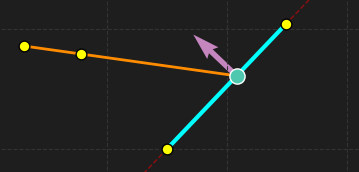
\includegraphics[width=\textwidth]{normal_OK}
        %\caption{Correct}
    \end{minipage}
    \hfill
    \begin{minipage}{0.45\textwidth}
        \centering
        {\Huge \textbf{\textcolor{red}{NO}}} \\ [0.5cm]
        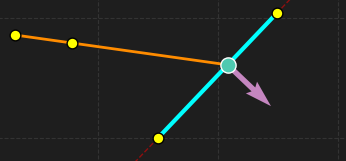
\includegraphics[width=\textwidth]{normal_wrong}
        %\caption{Incorrect}
    \end{minipage}
    \label{fig:normal_demo}
\end{figure}

\begin{center}
\renewcommand{\arraystretch}{2.0}
\begin{tabular}{r | c | c | c | c}
\toprule
\textbf{Math Symbol} & $\vec{d}$ & $\mathbf{P}_1$ & $\mathbf{P}_2$ & $\vec{n}$ \\
\midrule
\textbf{Argument} & \lstinline|ray_dir| & \lstinline|p1| & \lstinline|p2| & \lstinline|return| \\
\midrule
\textbf{Type} & \lstinline|np.array| & \lstinline|np.array| & \lstinline|np.array| & \lstinline|np.array| \\
\bottomrule
\end{tabular}
\end{center}
\textbf{Test:} Press "Reload \& Retest", than "L5 Line Normals" buttons in the visual debugger window. Ensure unittests are passing. Move different points in visual debugger and ensure your code works appropriately. Try reproducing the image in the problem description, ensure that the vector points appropriately.


\section*{Problem 6: Radial Orientation (Arc Normal)}

\subsubsection*{Mathematical part}
\textbf{Given:} The intersection point $\mathbf{Q}$ of the ray and the arc, the incident unit direction vector $\vec{d}$, and the arc's center $\mathbf{C}$.\\
\textbf{Derive:} The unit normal vector $\vec{n}$ at the hit point. Like the segment, the normal \textbf{must point against} the incident ray.

\subsubsection*{Implementation part}
\textbf{Implement:} a function \lstinline|calculate_normal_arc(hit_point, ray_dir, center)| that returns the unit normal vector $\vec{n}$ as a \lstinline|numpy.array|.

\begin{figure}[h]
    \centering
    \begin{minipage}{0.45\textwidth}
        \centering
        {\Huge \textbf{\textcolor{green}{OK}}} \\ [0.5cm]
        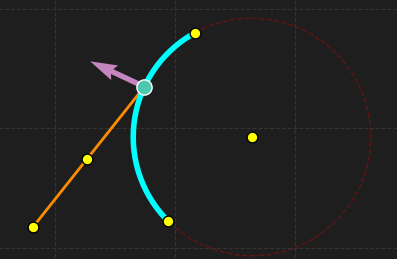
\includegraphics[width=\textwidth]{circle_OK}
        %\caption{Correct}
    \end{minipage}
    \hfill
    \begin{minipage}{0.45\textwidth}
        \centering
        {\Huge \textbf{\textcolor{red}{NO}}} \\ [0.5cm]
        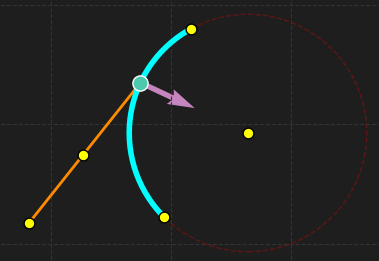
\includegraphics[width=\textwidth]{circle_NO}
        %\caption{Incorrect}
    \end{minipage}
    \label{fig:normal_demo}
\end{figure}

\begin{center}
\renewcommand{\arraystretch}{2.0}
\begin{tabular}{r | c | c | c | c}
\toprule
\textbf{Math Symbol} & $\mathbf{Q}$ & $\vec{d}$ & $\mathbf{C}$ & $\vec{n}$ \\
\midrule
\textbf{Argument} & \lstinline|hit_point| & \lstinline|ray_dir| & \lstinline|center| & \lstinline|return| \\
\midrule
\textbf{Type} & \lstinline|np.array| & \lstinline|np.array| & \lstinline|np.array| & \lstinline|np.array| \\
\bottomrule
\end{tabular}
\end{center}
\textbf{Test:} Press "Reload \& Retest", than "L6 Arc Normals" buttons in the visual debugger window. Ensure unittests are passing. Move different points in visual debugger and ensure your code works appropriately. Try reproducing the image in the problem description, ensure that the vector points appropriately.



\section*{Problem 7: Physical Optics (Refraction)}

\subsubsection*{Mathematical part}
\textbf{Given:} An incident unit direction vector $\vec{d}$, the unit normal vector $\vec{n}$ at the interface, and the refractive indices $n_1$ and $n_2$ of the two media. Suppose that the ray goes from the medium with $n_1$ into the medium with $n_2$. \\
\textbf{Derive:} The unit direction vector of the refracted ray $\vec{r}$. \textbf{Hint:} use the vector form of Snell's Law. First, find $\cos \theta_1$ and $\sin^2 \theta_1$ using the dot product. Then, calculate $\sin^2 \theta_2$ using the ratio $\eta = n_1/n_2$. If $\sin^2 \theta_2 > 1$, Total Internal Reflection (TIR) occurs and no refracted ray exists. Otherwise, derive $\vec{r} = \eta \vec{d} + (\eta \cos \theta_1 - \cos \theta_2)\vec{n}$.

\subsubsection*{Implementation part}
\textbf{Implement:} a function \lstinline|refract_vector(ray_dir, normal, n1, n2)| that returns the refracted unit vector $\vec{r}$ as a \lstinline|numpy.array|. If Total Internal Reflection occurs, return \lstinline|None|. \textbf{Note:} ensure that your normal $\vec{n}$ was correctly oriented.
\begin{center}
\renewcommand{\arraystretch}{2.0}
\begin{tabular}{r | c | c | c | c | c}
\toprule
\textbf{Math Symbol} & $\vec{d}$ & $\vec{n}$ & $n_1$ & $n_2$ & $\vec{r}$ \\
\midrule
\textbf{Argument} & \lstinline|ray_dir| & \lstinline|normal| & \lstinline|n1| & \lstinline|n2| & \lstinline|return| \\
\midrule
\textbf{Type} & \lstinline|np.array| & \lstinline|np.array| & \lstinline|float| & \lstinline|float| & \lstinline|np.array| or \lstinline|None| \\
\bottomrule
\end{tabular}
\end{center}
\textbf{Test:} Press "Reload \& Retest", than "L6 Refraction" buttons in the visual debugger window. Ensure unittests are passing. Move different points in visual debugger and ensure your code works appropriately. See if the light bends. \textbf{Debugger supposes that the light is always going from the air $n_1 = 1$ into the glass $n_2 = 1.5$.} Think if the beam should get closer of further from the normal, check in the visual debugger.


\section*{Problem 8: Run Physical Simulation}

Once you have verified your mathematical implementation using the unit tests and the Lab Dashboard, you are ready to observe the full physical simulation. Use the "Run Main Simulation" button to initialize the global ray tracer and observe how light interacts with the complex optical systems you have defined.

\subsubsection*{Navigating the Interface}
The simulation environment consists of several interactive components designed for real-time optical analysis:
\begin{itemize}
\item \textbf{The Optical Bench (Main Canvas):} This is your primary workspace where lenses and ray sources are visualized. You can interactively place, move, and rotate objects to alter the light path. Drag the lens with the left mouse button. Rotate the lens with the right mouse button. Use "n" at the top of the panel to set the refraction index. Parallel rays are going from the left;  you can change to point source and back with "Mode" button, point source is draggable with the left mouse button.
\item \textbf{Lens Architect:} Use this tool to define the geometry of your lenses. Drag colored points to change the lens shape. See parameters of the lens at the top. Note that a slab can be created.
\item \textbf{Physics Inspector:} Located in the side panel, this tool allows you to select individual lens to view its properties.
\item \textbf{Measurements:} Use "Ruler" button to go into measurement mode and back. When ruler is on you can measure distances by pressing left mouse button somewhere, dragging the mouse and releasing. You will see a line showing appropriate segment and the distance measured.
\item \textbf{Workspace Management:} You can save your current optical configuration or load predefined benchmarks using the \textbf{Save Lab/Load Lab} buttons.
\end{itemize}


\subsubsection*{Simulation Task}
\textbf{Execution:} Create a Keplerian telescope by placing two lenses of different focal lengths in the path of a parallel ray source. Observe the refraction at each interface. \\
\begin{center}
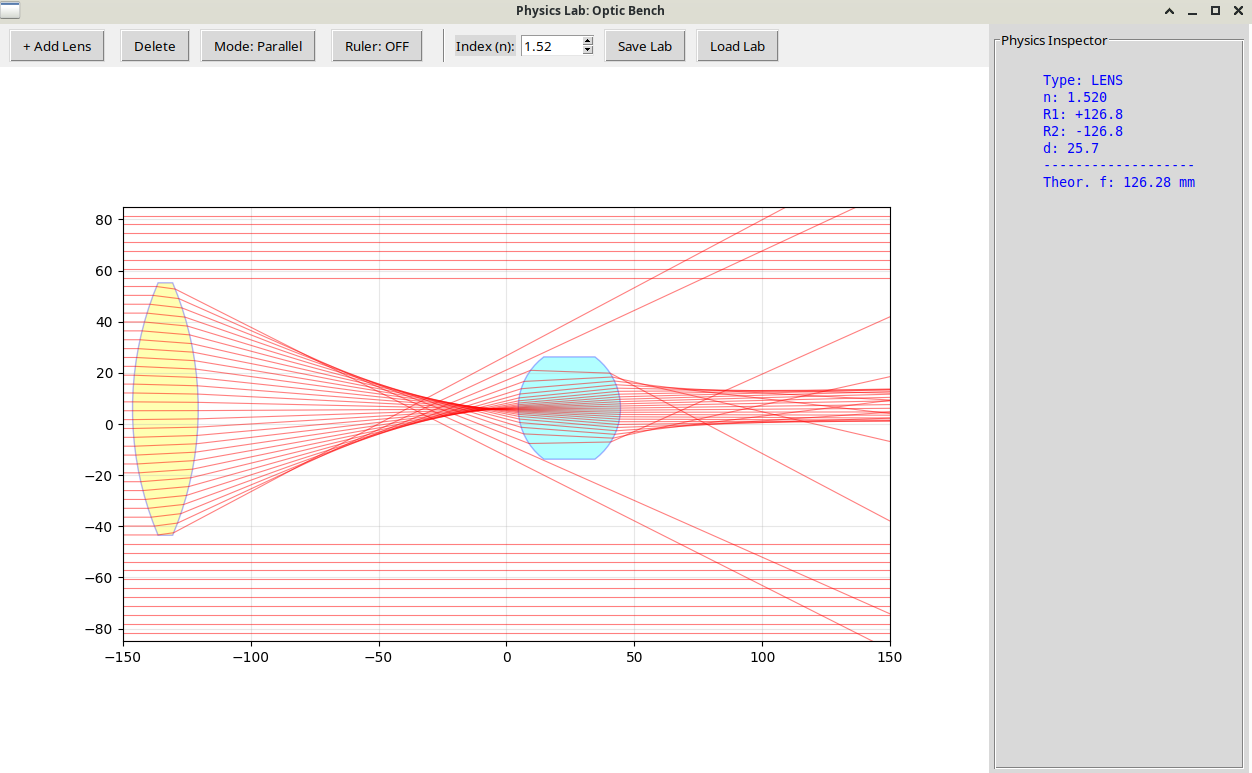
\includegraphics[width=0.7\textwidth]{telescope}
\end{center}


\section*{Problem 9: Lens Maker's Formula}

\subsubsection*{Implementation part}

\textbf{Task:} Implement \lstinline|calculate_focal_length(R1, R2, d, n)| that calculates the effective focal length $f$ for a thick lens using the standardized Gullstrand's form.
\textbf{Reference:} For the full derivation and sign convention rules, refer to the \href{https://en.wikipedia.org/wiki/Lens#Lensmaker's_equation}{Wikipedia: Lensmaker's equation}.The formula is given by:
$$
\frac{1}{f} = (n-1) \left[ \frac{1}{R_1} - \frac{1}{R_2} + \frac{(n-1)d}{n R_1 R_2} \right]
$$
\begin{center}
\renewcommand{\arraystretch}{2.0}
\begin{tabular}{r | c | c | c | c | c}
\toprule
\textbf{Math Symbol} & $R_1$ & $R_2$ & $d$ & $n$ & $f$ \\
\midrule
\textbf{Argument} & \lstinline|R1| & \lstinline|R2| & \lstinline|d| & \lstinline|n| & \lstinline|return| \\
\midrule
\textbf{Type} & \lstinline|float| & \lstinline|float| & \lstinline|float| & \lstinline|float| & \lstinline|float| \\
\bottomrule
\end{tabular}
\end{center}

\subsubsection*{Experimentation part}

\textbf{Task:} Add any lens to the field, see that Physics inspector now shows the focal lengths (if not - check implementation). Using parallell mode, determine the position of he focus, set "Ruler:ON" and measure the distance. It is expected that distance will be approximately equal to the one you have calculated (shown in Physics Inspector).
\begin{center}
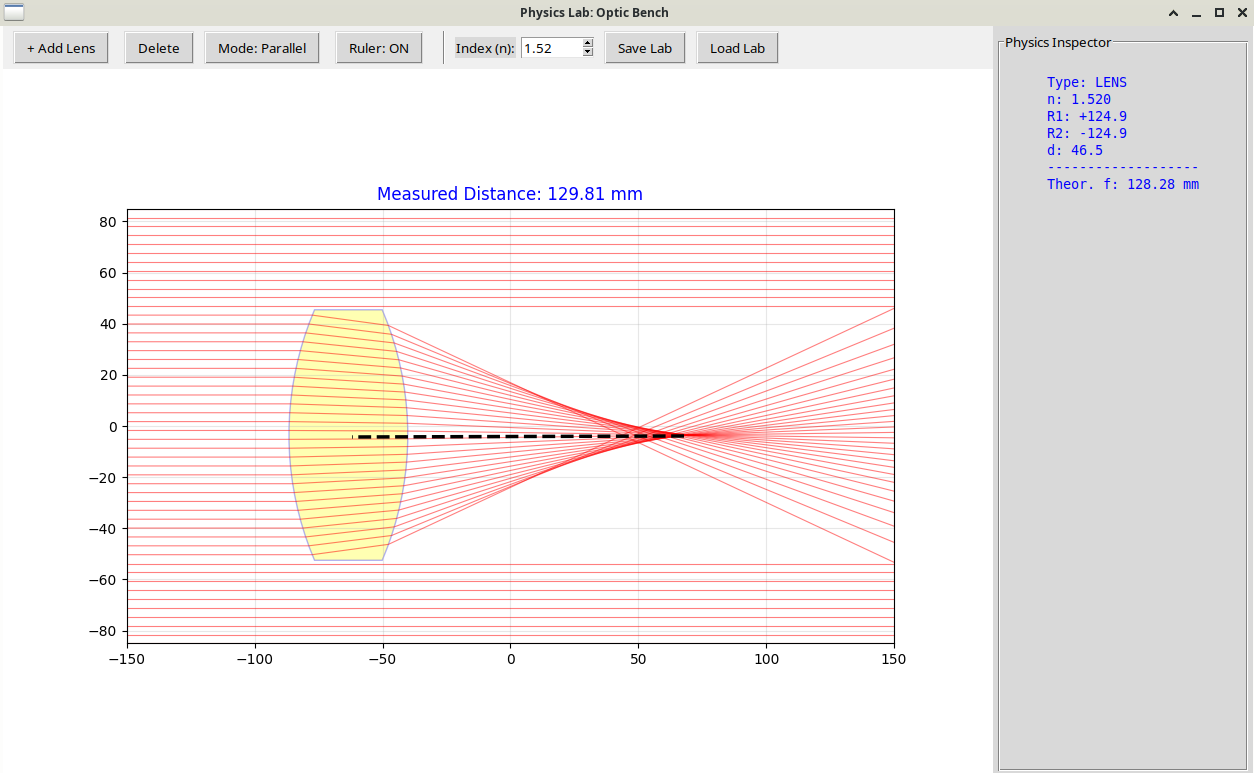
\includegraphics[width=0.7\textwidth]{focus_dist}
\end{center}

\textbf{Note:} Actual focal distances should be measured to optical planes, but we assume our lenses thin (despite calculate focus assuming them thick). This introduces certain measurement error, but we ignore it for now.


\section*{Problem 10: Lateral Shift (Parallel Slab)}

\subsubsection*{Implementation part}
\textbf{Task:} Implement \lstinline|calculate_slab_displacement(d, n, theta)| that determines the lateral displacement $h$ of a ray passing through a transparent slab.\textbf{Reference:} For the geometric derivation and the relationship between incident and refracted angles, refer to the \href{https://en.wikipedia.org/wiki/Snell\%27s_law#Vector_form}{Wikipedia: Displacement by a parallel plate}. The formula is:
$$
h = d \frac{\sin(\theta - \theta')}{\cos \theta'},
$$
where $\theta$ is the incident angle and $\theta'$ is the refracted angle derived from Snell's Law ($n \sin \theta' = \sin \theta$).
\begin{center}
\renewcommand{\arraystretch}{2.0}
\begin{tabular}{r | c | c | c | c}
\toprule
\textbf{Math Symbol} & $d$ & $n$ & $\theta$ & $h$ \\
\midrule
\textbf{Argument} & \lstinline|d| & \lstinline|n| & \lstinline|theta| & \lstinline|return| \\
\midrule\textbf{Type} & \lstinline|float| & \lstinline|float| & \lstinline|float| & \lstinline|float| \\
\bottomrule
\end{tabular}
\end{center}

\subsubsection*{Experimentation part}
\textbf{Task:} Place a glass slab (or a rectangular lens defined by segments) into the path of parallel rays. Rotate the slab to create an incident angle $\theta$. View angle and expected displacement $h$ in the Physics Inspector. Using the "Ruler" tool, measure the perpendicular distance between the path of the incident ray and the path of the exiting ray.
\begin{center}
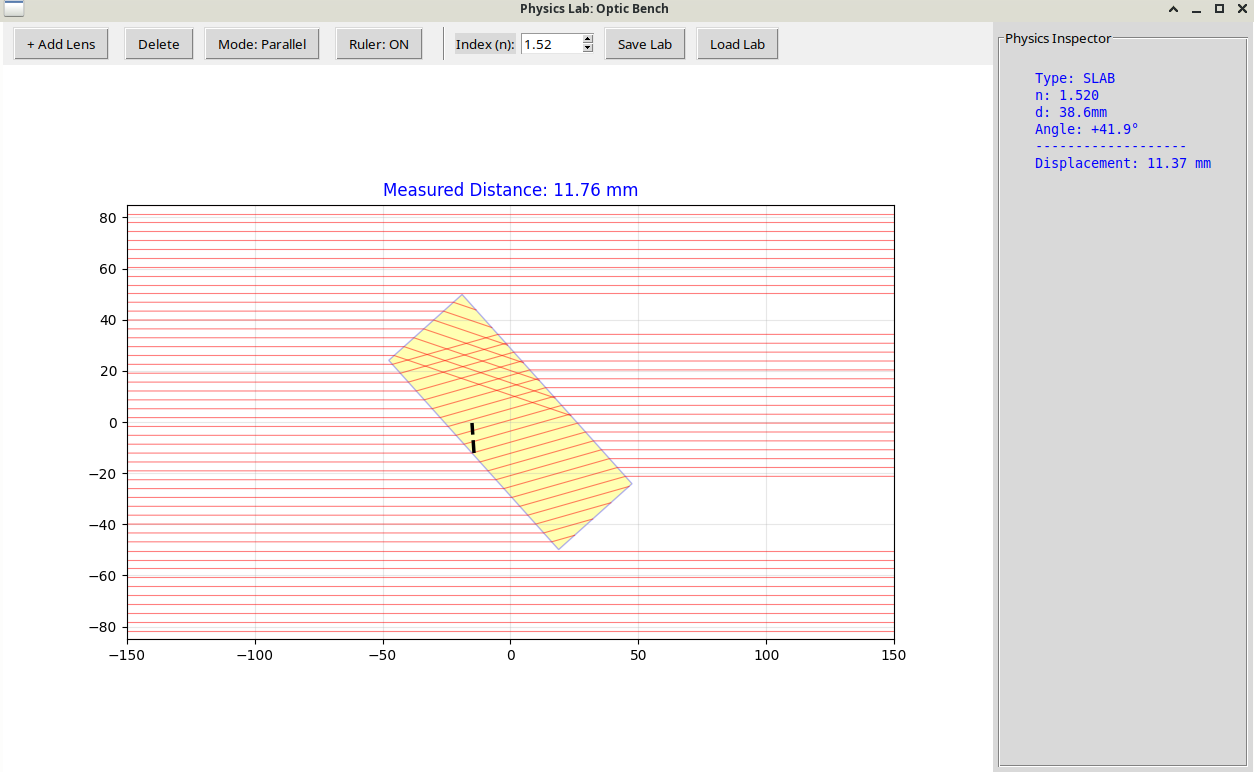
\includegraphics[width=0.7\textwidth]{displacement}
\end{center}


\section*{\textcolor{red}{Submission}}

Submit the file \texttt{implementation\_tasks.py} and the screenshots for experimental problems.


\end{document}
